%%%%%%%%%%%%%%%%%%%%%%%%%%%%%%%%%%%%%%%%%%%%%%%%%%%%%%%%%%%%%%%%%%%%%%%%%%%%%%%
% CAPÍTULO 4 - PROPUESTA DE DISEÑO DEL SITIO WEB DEL PROYECTO
%%%%%%%%%%%%%%%%%%%%%%%%%%%%%%%%%%%%%%%%%%%%%%%%%%%%%%%%%%%%%%%%%%%%%%%%%%%%%%%
\chapter{Propuesta de diseño del sitio web del proyecto}
\label{chap:webProp}
Tras la gestión necesaria que necesita un paquete de software desarrollado en Python. En el presente capítulo se muestra la solución web para el software desarrollado de PyCardio, donde trataremos de mostrar las partes que la componen y como han sido implementadas.

Para mostrar la web, el proceso que seguirá esta memoria es la de ir sección por sección donde enseñamos tanto el resultado como la implementación que sigue.

Antes de comenzar, debemos destacar que dicha web se ha implementado utilizando una plantilla adquirida por el equipo de la universidad y diseñada por el equipo WrapBootstrap, esta plantilla se la conoce en dicho servicio como Unify. 

%%%%%%%%%%%%%%%%%%%%%%%%%%%%%%%%%%%%%%%%%%%%%%%%%%%%%%%%%%%%%%%%%%%%%%%%%%%%%%%%%%%%%%%%%%
%                       HOME
%%%%%%%%%%%%%%%%%%%%%%%%%%%%%%%%%%%%%%%%%%%%%%%%%%%%%%%%%%%%%%%%%%%%%%%%%%%%%%%%%%%%%%%%%%
\section{Home}
\label{sec:homeWeb}
Nada más entrar en la web de PyCardio, entramos en el home de la página. El Home se ha implementado de manera que sea lo más visual y sencillo para el usuario, de modo que nada más entrar se nos ofrece la interfaz de todas las secciones, una breve descripción de que es PyCardio, y los enlaces para redirigirnos a la documentación alojada en Read The Docs y al código de software a la última release alojada en GitHub. 

\begin{figure}[H]
    \centering
    \subfloat[Home 1]{
        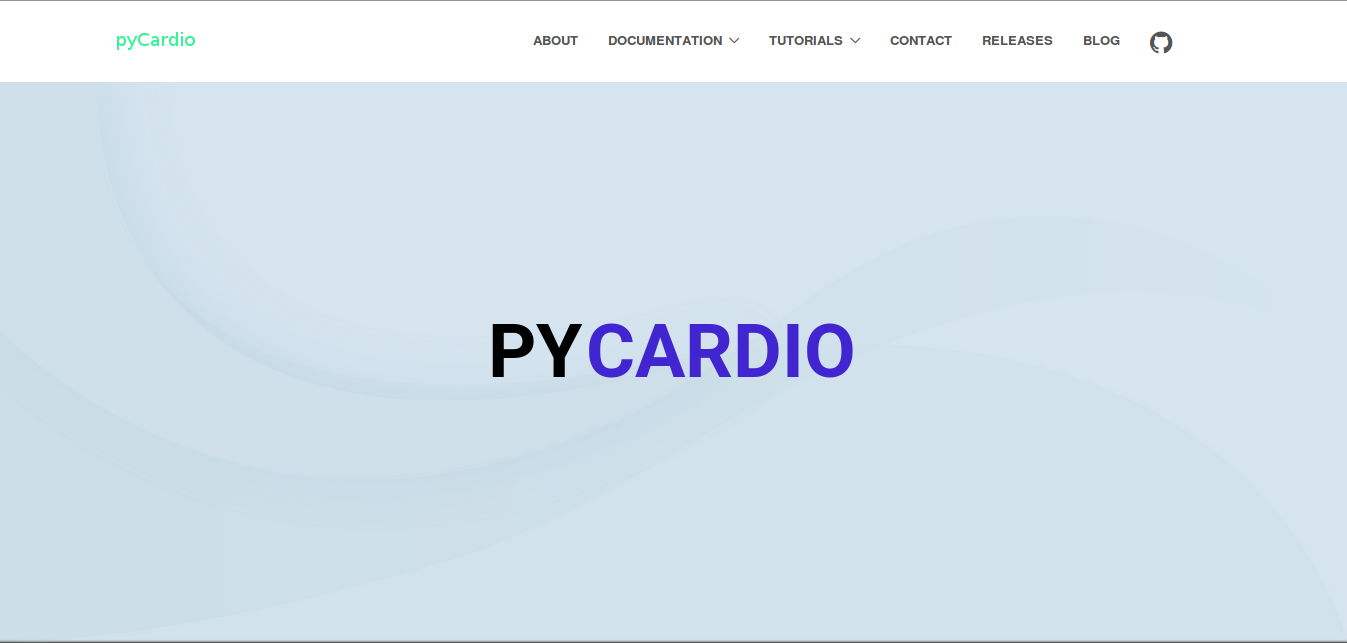
\includegraphics[width=0.3\textwidth]{img/home_1.png}
        \label{fig:home1}
        }
    \subfloat[Home 2]{
        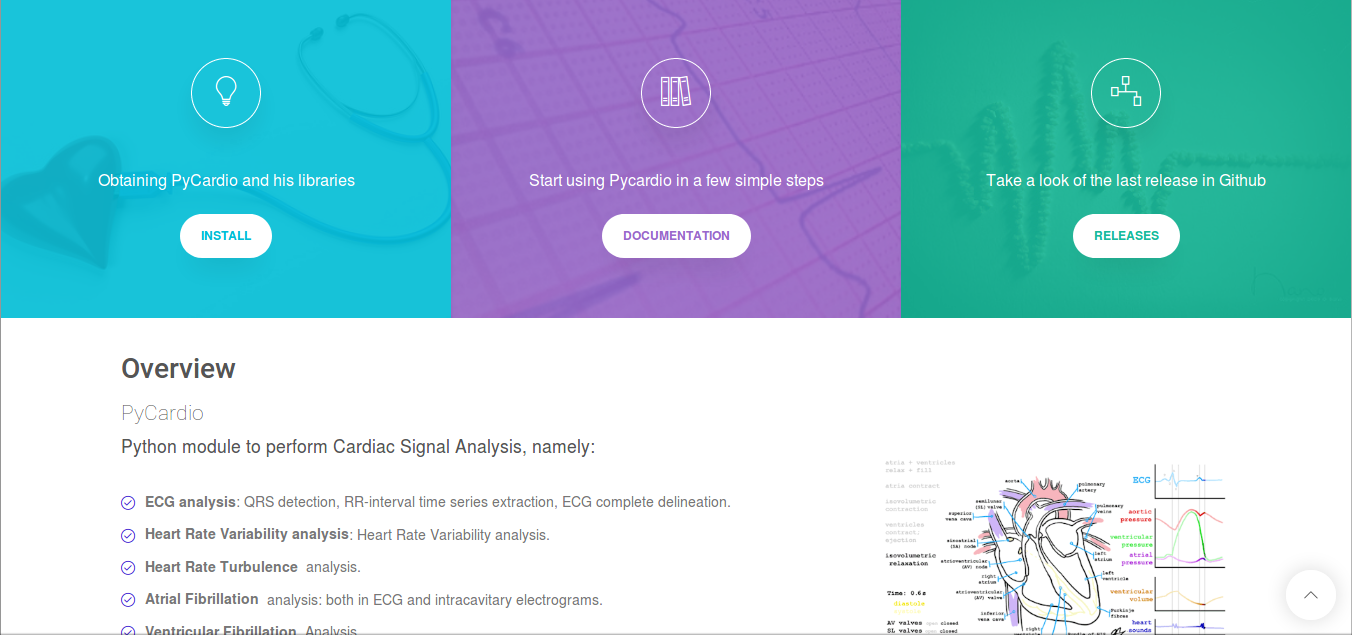
\includegraphics[width=0.3\textwidth]{img/home_2.png}
        \label{fig:home2}
    }
    \subfloat[Home 3]{
        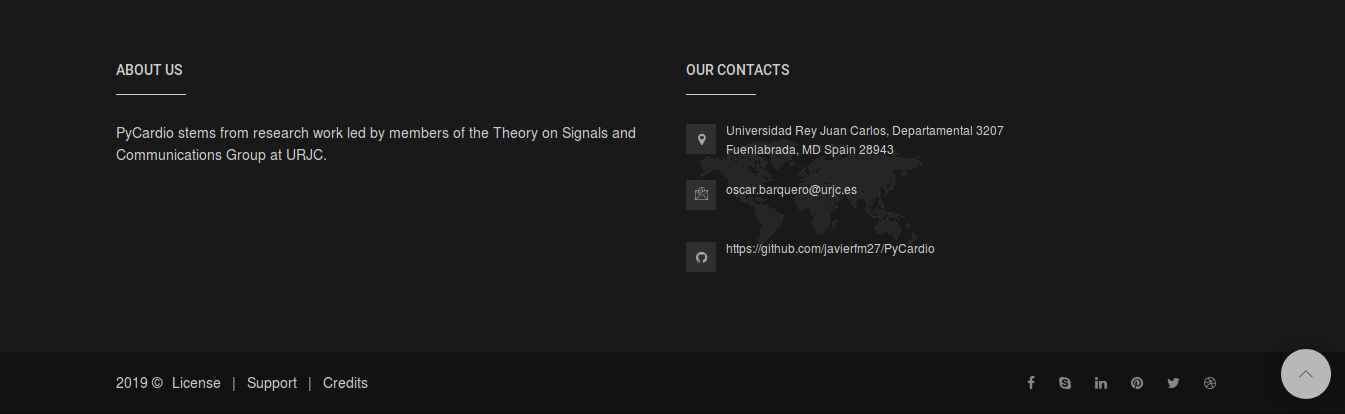
\includegraphics[width=0.3\textwidth]{img/home_3.png}
        \label{fig:home3}
    }
    \caption{Home de PyCardio}
    \label{fig:homePyCardio}
\end{figure}

Para su implementación, lo primero que se realiza es la creación de un fichero \texttt{index} en la raíz del proyecto, donde Jekyll interpretará que dicho fichero será el HTML principal de la web. El fichero puede ser escrito como ya se ha comentado, en MarkDown o en lenguaje de marcado HTML, en nuestro caso, MarkDown. El fichero solo se compone de un Front Matter en el que se llama al layout de Main, y en el que proporciona el título de la página principal.
\begin{lstlisting}[language=yaml,caption=index.md. Fichero de home de PyCardio,label=co]
    ---
layout: main
title: PyCardio Home
    ---
\end{lstlisting}

El contenido del layout; main, se compondrá de lenguaje HTML. Este contenido además se rellena con los mencionados \textbf{includes} en el \ref{subsec:githubJekyll}, que compondrá aquel código que se repetirá en todas las secciones de la web, permitiendo así centralizar el desarrollo, de manera que, si quisiéramos cambiar el contenido de estos componentes solo tendríamos que realizar dicho cambio en un solo fichero. Para el desarrollo de este prototipo web, se han distinguido los siguientes:
\begin{itemize}
    \item \textbf{\texttt{css.html}}: En él se incluyen todos los enlaces a los archivos CSS necesarios para la presentación final de la web.
    \item \textbf{\texttt{js.html}}: Incluye los enlaces a los archivos necesarios para el contenido de la web que hace uso de JavaScript.
    \item \textbf{\texttt{header.html}}: Contiene el panel de navegación de todas las secciones de la web.
    \item \textbf{\texttt{footer.html}}: Parte final de todas las páginas que componen la web. En ella se incluye la licencia a la que está el software, enlaces a las redes sociales del proyecto, y enlace a soporte.
    \item \textbf{\texttt{breadc.html}}: Compone el camino en el que nos encontramos dentro de la web. En el hacemos uso del lenguaje Liquid, para poder construir dicho contenido. 
\end{itemize}

Si observamos las imágenes de la figura \ref{fig:homePyCardio} podemos ver que en el layout referenciado, main, tendremos los includes de \texttt{footer.html} y \texttt{header.html}, además de los de CSS y Javascript, que estos procurarán ir en todas las páginas de la web. 

\begin{figure}[H]
    \centering
    \subfloat[header]{
        
\includegraphics[width=0.3\textwidth]{img/header.png}
        \label{fig:includHeader}
        }
    \subfloat[breadcrumber]{
        
\includegraphics[width=0.3\textwidth]{img/breadc.png}
        \label{fig:includBread}
    }
    \subfloat[footer]{
        
\includegraphics[width=0.3\textwidth]{img/footer.png}
        \label{fig:includFooter}
    }
    \caption{Includes de PyCardio}
    \label{fig:includ}
\end{figure}

Así, el Home de la web al ser una página única que no va a tener parecido alguno en lo restante de web excepto en los \texttt{includes} mencionados, el propio layout main, es la página desarrollada, por esto \texttt{index.md} solo se compone de la llamada a dicha plantilla y del título. 

Antes de pasar a tratar la siguiente sección de la web, cabe mencionar, que se crea un \texttt{include} más, denonminado \texttt{script.html}, donde irá al final de los layouts desarrollados, que contendrán aquella tecnología JQuery y Javascript que utiliza la plantilla para hacer de la web   ``sensible'' o como llamamos hoy en día a este tipo de webs \textit{responsive}.
%%%%%%%%%%%%%%%%%%%%%%%%%%%%%%%%%%%%%%%%%%%%%%%%%%%%%%%%%%%%%%%%%%%%%%%%%%%%%%%%%%%%%%%%%%
%                       ABOUT
%%%%%%%%%%%%%%%%%%%%%%%%%%%%%%%%%%%%%%%%%%%%%%%%%%%%%%%%%%%%%%%%%%%%%%%%%%%%%%%%%%%%%%%%%%
\section{About}
\label{sec:aboutWeb}
Esta sección de la web trata de dar una vista general de todos aquellos que han formado parte del proyecto PyCardio, tanto para su parte de desarrollo de software como en la parte de implementación de la web. 

\begin{figure}[H]
    \centering
    \subfloat[About 1]{
        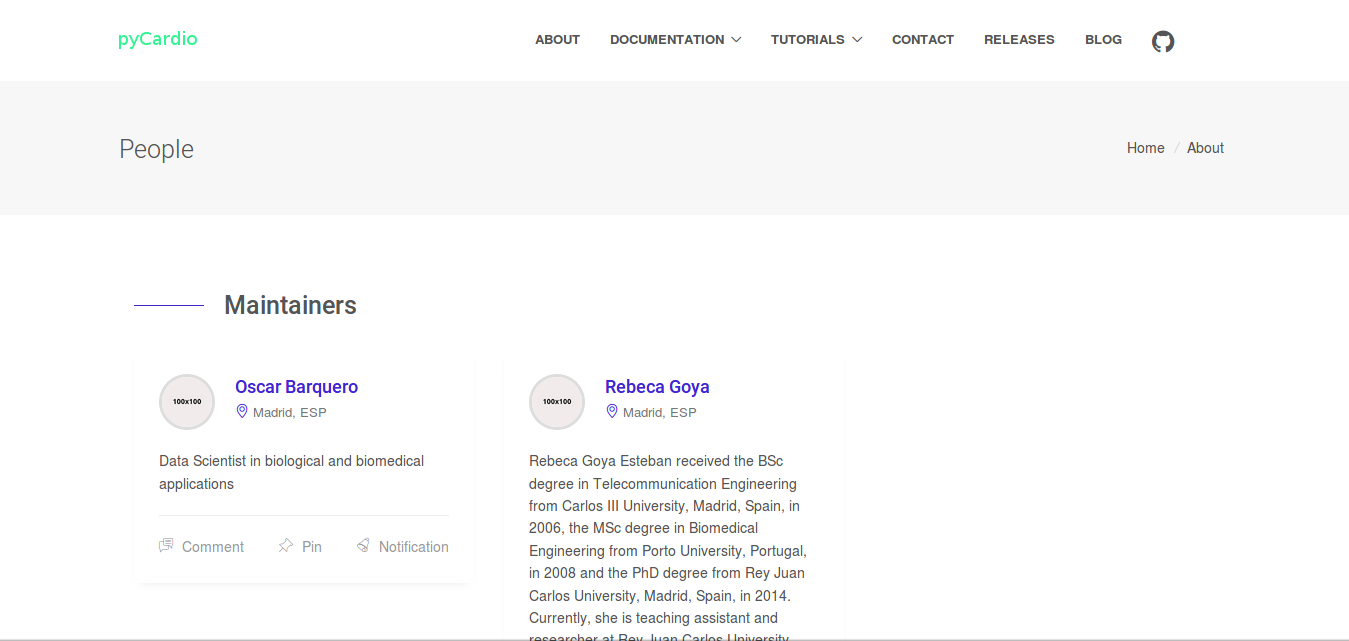
\includegraphics[width=0.5\textwidth]{img/about_1.png}
        \label{fig:aboutWeb1}
    }
    \subfloat[About 2]{
        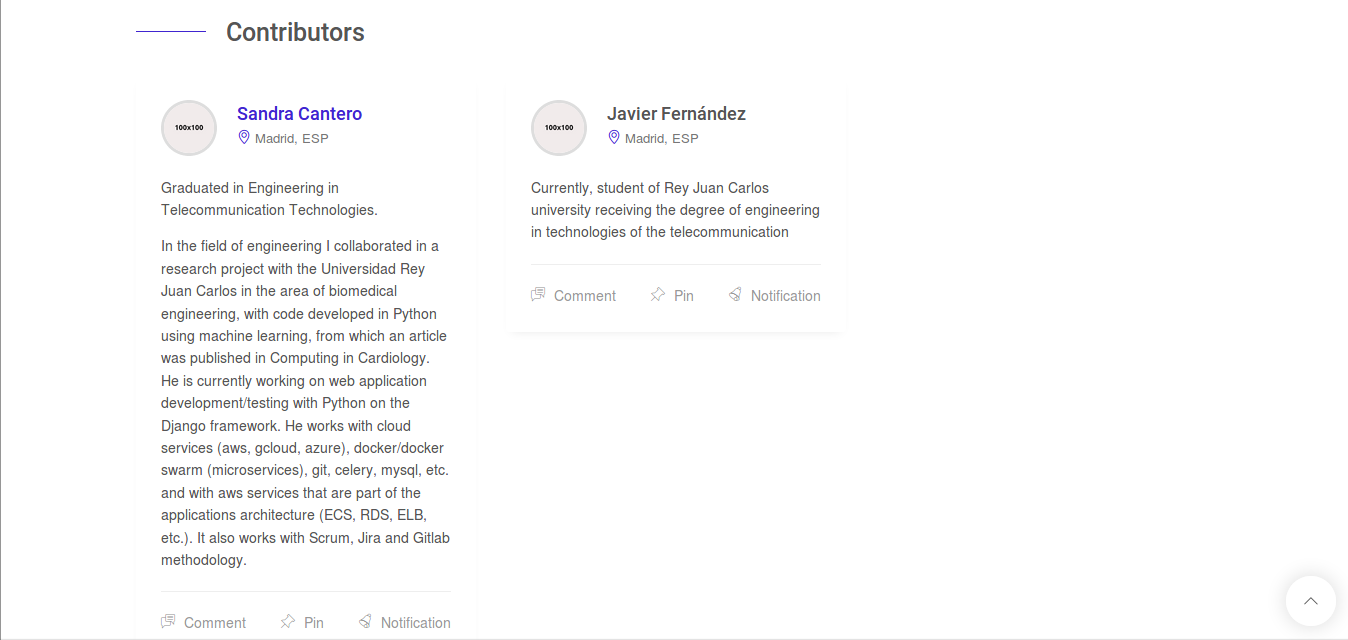
\includegraphics[width=0.5\textwidth]{img/about_2.png}
        \label{fig:aboutWeb2}
    }
    \caption{Sección About de la web PyCardio}
    \label{fig:aboutWeb}
\end{figure}

Para su implementación se ha diseñado un nuevo layout denominado \texttt{page.html} y es el dado por el listing \ref{code:layoutPage}, que será el utilizado para la mayoría de las páginas que se quieran añadir a la web. Tanto Jekyll como nosotros en el desarrollo de PyCardio Web, hacemos una distinción entre dos tipos de páginas:

\begin{itemize}
    \item \textbf{Pages: } Las páginas es aquel contenido que no está basado en una fecha.
    \item \textbf{Posts: } Aquel contenido que se distingue por la fecha en la que se publicó en la web.
\end{itemize}

\begin{lstlisting}[style=htmlcssjs,caption=Layout Page,label={code:layoutPage}]
<!DOCTYPE html>
<html lang="en">
<head>
  <!-- Title -->
  <title>{{page.title}} | PyCardio</title>

  <!-- Required Meta Tags Always Come First -->
  <meta charset="utf-8">
  <meta name="viewport" content="width=device-width, initial-scale=1, shrink-to-fit=no">
  <meta http-equiv="x-ua-compatible" content="ie=edge">

  <!-- Google Fonts -->
  <link href="https://fonts.googleapis.com/css?family=Open+Sans:300,400,600,700,800" rel="stylesheet">

  
  <meta http-equiv="refresh" content="5; url=/">
  


  
  

</head>

<body>
  
  
  

  <div class="container g-mt-50 g-mb-60">
    {{ content }}
  </div>

  

  
</body>
\end{lstlisting}

Para la implementación de \textit{About}, nuestra página hará referencia al \textit{layout}\texttt{page.html} y el contenido se incrustará en la variable del lenguaje de plantilla Liquid denominada \texttt{content}. Al incluir \textit{shortcodes}\footnote{Trozos de código que utiliza los plugins que en este caso vienen junto con la plantilla Unify adquirida.} de la plantilla Unify, el contenido que tendrá nuestro fichero principal de la sección \textit{about} será HTML.

El \textit{shortcode} utilizado trata de un elemento de bloque en el que solo hace uso de los CSS que vienen junto con la plantilla. Quedando así tal y como lo muestra el listing \ref{code:about}. 
\begin{lstlisting}[style=htmlcssjs,caption=index.html de About,label={code:about}]
---
layout: page
title: People
---
<div class="container">
  <br>
  <!-- HEADING  MAINTAINERS-->
  <div class="shortcode-html">
    <div class="u-heading-v6-2 g-mb-20">
      <h2 class="h3 u-heading-v6__title g-brd-primary">Maintainers</h2>
    </div>
  </div>
  <!-- END HEADING MAINTAINERS-->

  <!-- TEAM BLOCK -->
  <div class="row">
    <div class="col-lg-4 g-mb-30">
      <!-- Figure -->
      <figure class="u-shadow-v19 g-bg-white g-rounded-4 g-pa-25">
        <div class="media g-mb-20">
          <div class="d-flex g-mr-20">
            <!-- Figure Image -->
            <div class="g-brd-around g-brd-3 g-brd-gray-light-v3 rounded-circle">
              <img class="rounded-circle g-width-50 g-height-50" src="../../assets/img-temp/100x100/img7.jpg" alt="Image Description">
            </div>
            <!-- Figure Image -->
          </div>
          <div class="media-body">
            <!-- Figure Info -->
            <h4 class="h5 g-mb-2"><a href="https://gestion2.urjc.es/pdi/ver/oscar.barquero#tab_1_5">Oscar Barquero</a></h4>
            <div class="d-block">
              <i class="g-color-primary g-font-size-default icon-location-pin"></i>
              <span class="g-color-gray-dark-v4 g-font-size-13">Madrid, ESP</span>
            </div>
            <!-- End Figure Info -->
          </div>
        </div>

        <p>Data Scientist in biological and biomedical applications</p>
      </figure>
      <!-- End Figure -->
    </div>
\end{lstlisting}

Antes de continuar seguramente os habréis preguntado el por qué de otro fichero \texttt{index} si ya habíamos diseñado uno para el \texttt{home} de nuestra web. Esto es porque cuando tenemos varias páginas en nuestra página web, lo más eficaz es seguir un orden en los directorios, en consecuencia si estamos desarrollando la sección \texttt{about}, tengamos en un directorio \texttt{/about/}, todos aquellos contenidos que compondrán esta sección. De manera que, para Jekyll, el fichero en el directorio \texttt{/about/index.html}, será el fichero principal para esa sección.

Así si escribimos un hiperenlace en nuestro web escribiendo \texttt{\{\{site.url\}\}/about/} \footnote{\texttt{\{\{site.url\}\}} es una variable del \textit{framework} Jekyll definido en el fichero de configuración(\texttt{config.yml}) donde obtenemos la dirección URL del sitio web}, nos mostrará el contenido generado por \texttt{index.html}, en nuestro directorio \texttt{/about/}.

Si comparamos los dos \textit{layouts} de los que disponemos vemos que en el nuevo introducido por esta sección, hacemos uso del \textit{include} de \texttt{breadc.html} donde hacemos uso de la variable \texttt{page}, que brinda información de página específico y permite el uso de las variables definidas en el Front Matter y de setencias de control del lenguaje de plantilla Liquid.   

\begin{lstlisting}[style=htmlcssjs,caption=Breadcrumber,label={code:breadcrum}]
  <div class="align-self-center ml-auto">
          <ul class="u-list-inline">
            <li class="list-inline-item g-mr-5">
              <a class="u-link-v5 g-color-main" href="{{site.url}}">Home</a>
              <i class="g-color-gray-light-v2 g-ml-5">/</i>
            </li>
            
            
            

               
                
                  <li class="list-inline-item g-mr-5">
                  {{page.title}}
                  </li>
                
              
                <li class="list-inline-item g-mr-5">
                  <a class="u-link-v5 g-color-main">{{ element |capitalize }}</a>
                  

                  
                    <i class="g-color-gray-light-v2 g-ml-5">/</i>
                  
                </li>
              

            
          </ul>
        </div>
\end{lstlisting}

